\documentclass{beamer}
\usetheme{Frankfurt}
\usepackage[utf8]{inputenc}
\usepackage{charter}
\usepackage{tikz}
\usepackage{graphicx}
\usepackage{amsmath}
\usepackage{amssymb}
\usepackage{listings}
\usepackage{animate}
\usepackage{bm}
\beamertemplatenavigationsymbolsempty

\let\vec\bm

%% Title slide formatting %%

\pgfdeclareimage[width=\paperwidth]{titlebackground}{Images/title-slide-background.png}
\setbeamerfont{subtitle}{size=\tiny}
\setbeamertemplate{endpage}{
	\begin{picture}(0,0)
		\scalebox{1.01}{
		\put(-28.5,-163){%
			\pgfuseimage{titlebackground}
		}
		}
		\put(0,-115){%
			\begin{minipage}[b][4.5cm][t]{0.5\textwidth}
				\color{white}
				\usebeamerfont{title}
				{\textbf{Thank Your} \\ \textbf{For You Attention !}}
			\end{minipage}
		}
	\end{picture}
}
\setbeamertemplate{title page}{
	\begin{picture}(0,0)
		\scalebox{1.01}{
			\put(-28.5,-163){%
				\pgfuseimage{titlebackground}
			}
		}
		\put(0,-75){%
			\begin{minipage}[b][4.5cm][t]{0.5\textwidth}
				\color{white}
				\usebeamerfont{title}
				{\inserttitle\\[0.9cm]}
				\usebeamerfont{subtitle}
				{\insertauthor\par}
				{\insertinstitute\\[0.3cm]}
				{\insertdate}
			\end{minipage}
		}
	\end{picture}
}


%% General slide formatting %%

\definecolor{oxfordblue}{RGB}{4,30,66}

\pgfdeclareimage[width=0.9cm]{oxfordlogo}{Images/oxford-logo.png}
\pgfdeclareimage[width=1cm]{mathslogo}{Images/mathematics-logo.png}
\pgfdeclareimage[width=0.9cm]{pizzalogo}{Images/pizza-logo.png}

\setbeamertemplate{headline}
{%
	\begin{picture}(0,0)
		\put(314,-50){%
			\pgfuseimage{oxfordlogo}
		}
		\put(20,-55){%
			\rule{320pt}{0.4pt}
		}
	\end{picture}
}

\setbeamertemplate{frametitle}
{%
	\begin{picture}(0,0)
		\put(-8,-20){%
			\normalsize\textbf{\color{oxfordblue}\insertframetitle}
		}
		\put(-7,-25){%
			\small\color{oxfordblue}\insertframesubtitle
		}
	\end{picture}
}

\setbeamertemplate{footline}
{%
	\begin{picture}(0,0)
		\put(20,30){%
			\rule{320pt}{0.4pt}
		}
		\put(20,14){%
			\pgfuseimage{mathslogo}
		}
		\put(100,14){%
			\color{oxfordblue}\insertshortdate
		}
		\put(160,14){%
			\color{oxfordblue}\insertshorttitle
		}
		\put(337,14){%
			\color{oxfordblue}\insertpagenumber
		}
	\end{picture}%
}
\setbeamercolor{block title}{bg=oxfordblue!30,fg=black}

\definecolor{codegreen}{rgb}{0,0.6,0}
\definecolor{codegray}{rgb}{0.5,0.5,0.5}
\definecolor{codepurple}{rgb}{0.58,0,0.82}
\definecolor{backcolour}{rgb}{0.95,0.95,0.92}

\lstdefinestyle{mystyle}{
	%backgroundcolor=\color{backcolour},   
	commentstyle=\color{codegray},
	keywordstyle=\color{oxfordblue},
	numberstyle=\tiny\color{codegray},
	stringstyle=\color{codegreen},
	basicstyle=\ttfamily\footnotesize,
	breakatwhitespace=false,         
	breaklines=true,                 
	captionpos=b,                    
	keepspaces=true,                 
	numbers=left,                    
	numbersep=5pt,                  
	showspaces=false,                
	showstringspaces=false,
	showtabs=false,                  
	tabsize=2
}

\lstset{style=mystyle}

%% Information (author, title, etc.) %%
\title[Acoustic Rarefied Nematic Liquid Crystals]{Anisotropic Acoustic \vspace{0.1cm}\\ Waves In Rarefied Nematic\\ \\Liquid Crystals} % short title for footer
\author%
{%
	\sc{P. E. Farrell} *,\underline{\sc{U. Zerbinati}} *\\
}
\institute%
{%
	* \textit{Mathematical Institute}\\
	\;\textit{University of Oxford}\\
}

\date[Firedrake 2023]{22nd GAMM Seminar on Microstructures, 27th of January 2023, Vienna} % short date for footer



%% Content of slides %%

\begin{document}
	\begin{frame}[plain]
		\titlepage
	\end{frame}
	%
	\begin{frame}
		\frametitle{Why Rarefied Nematic Liquid Crystal ?}
		\begin{minipage}{0.49\textwidth}
			\vspace{0.8cm}
			\begin{figure}
				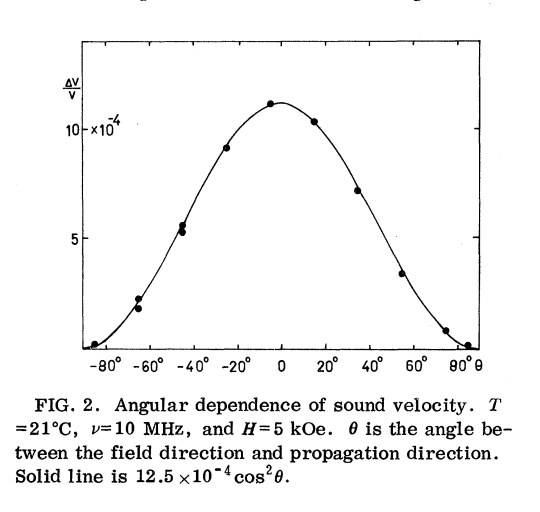
\includegraphics[scale=0.25]{Figures/MullenLuthiStephen}
				\vspace{-0.4cm}
				\caption{It was observed in \cite{MullenEtAll} that acoustic waves travel in NLC faster in the direction parallel to the nematic director.}
			\end{figure}
		\end{minipage}
		\begin{minipage}{0.49\textwidth}
			\vspace{1cm}
			\begin{figure}
				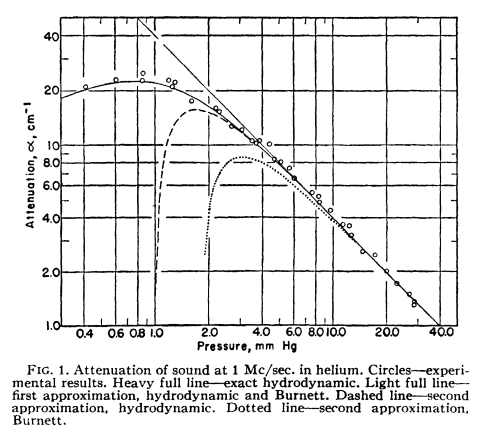
\includegraphics[scale=0.25]{Figures/Greenspan}
				\caption{It was observed in \cite{Greenspan} that first order theory better fit experimental data on acoustic attenuation at low pressure.}
			\end{figure}
		\end{minipage}
	\end{frame}
	\begin{frame}
		\frametitle{Curtiss Collision Operator}
		$\newline$
		Curtis in his seminal paper \cite{Curtiss} proposed a kinetic theory for spherocylindrical molecules as an idealisation of polyatomic gas.
		\\
		$\newline$
		\begin{minipage}{0.7\textwidth}
			\begin{itemize}
				\item[\color{oxfordblue}$\blacktriangleright$] His considered a larger configuration space made by \textbf{position}, \textbf{velocity}, \textbf{Euler's angles} for describing the orientation of each molecules and the \textbf{angular velocity} with respect to a fixed coordinate system.
				\item[\color{oxfordblue}$\blacktriangleright$] Molecules would interact by \textbf{excluded volume}, which give rise to \textbf{short range interactions} hence the \textbf{nematic ordering}.
			\end{itemize}
		\end{minipage}
		\qquad
		\begin{minipage}{0.2\textwidth}
			\begin{figure}
				\centering
				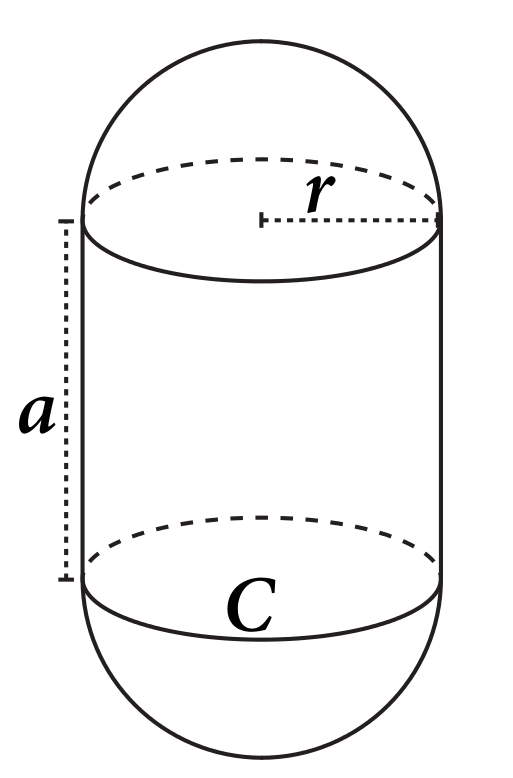
\includegraphics[scale=0.15]{Figures/spherocylinder}
			\end{figure}
		\end{minipage}
	\end{frame}
	\begin{frame}
		$\newline$
		$\newline$
		$\newline$
		This led Curtiss to formulate the following \textbf{Boltzmann} type equation,
		\begin{equation}
			\partial_t f + \nabla_{\vec{r}}\cdot(\vec{v}f)+\nabla_{\vec{\alpha}}\cdot(\dot{\vec{\alpha}}f) = C[f,f]
		\end{equation}
		where $f(\vec{r},\vec{v},\vec{\alpha},\vec{\omega})$ is the usual first reduced distribution function and $C[f,f]$ is the collision operator defined as
		\begin{equation}
			C[f,f] = - \int\int\int\int (f_1^{'}f^{'}-f_1f)(\vec{k}\cdot\vec{g})S(\vec{k})d\vec{k}d\vec{v}_1d\vec{\alpha}_1d\vec{\omega}_1
		\end{equation}
		with $\S(\vec{k})d\vec{k}$ being the surface element of the excluded volume and $\vec{g}=\vec{v}-\vec{v}_1$.
		Here with out loss of generality the equation is stated in \textbf{absence of external force} and \textbf{torque}.
	\end{frame}
	\begin{frame}[t, allowframebreaks]
		\frametitle{References}
		$\newline$
		$\newline$
		\bibliographystyle{amsalpha}
		\bibliography{metrix}
	\end{frame}
\end{document}
